\documentclass{beamer}

\usepackage{../Research}

\newcommand{\F}{\mathcal F}
\newcommand{\curly}[1]{\left\{ #1 \right\}}


\title{A Tiny Example}
\author{Andrew Mertz and William Slough}
\date{June 15, 2005}


\begin{document}

\maketitle

\begin{frame}
	Suppose we have an (infinite) collection of sets $\F$. \\
	We define a shatter function $\pi_\F(n)$

	\begin{align*}
		\pi_\F(n) = \max \{ &\text {\# of atoms in boolean algebra generated by $S$} \\
		            &\mid S \subset \F \text{ with } |S| = n\}
	\end{align*}
\end{frame}

\begin{frame}
	Example: Let $\F$ consist of all discs on a plane.
	\begin{figure}[p]
    \centering
    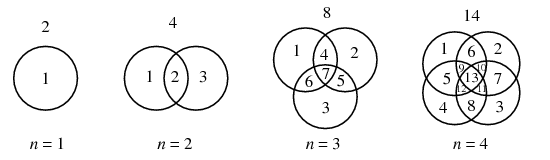
\includegraphics[scale=0.75]{circle.png}
	\end{figure}
	\begin{align*}
		\pi_\F(1) = 2 \ \ \  \pi_\F(2) = 4 \ \ \  \pi_\F(3) = 8  \ \ \ \pi_\F(4) = 14
	\end{align*}
	\begin{align*}
		\pi_\F(n) = n^2 - n + 2
	\end{align*}
\end{frame}

\begin{frame}
More examples: \\
	\begin{enumerate}
		\item Lines on a plane $\pi_\F(n) = n^2/2 + n/2 + 1$
		\item Disks on a plane	$\pi_\F(n) = n^2 - n + 2$
		\item Balls in $\R^3$  $\pi_\F(n) = n^3/3 - n^2 + 8n/3$
		\item Intervals on a line $\pi_\F(n) = 2n$
		\item Half-planes on a plane $\pi_\F(n) = n(n+1)/2 + 1$
		\item Finite subsets of $\N$ $\pi_\F(n) = 2^n$
		\item Polygons in a plane $\pi_\F(n) = 2^n$
	\end{enumerate}
\end{frame}

\begin{frame}
	\begin{Theorem} [Sauer-Shelah]
		Shatter function is either $2^n$ or bounded by a polynomial.
	\end{Theorem}
	\begin{Definition}
		Suppose growth of shatter function for $\F$ is polynomial.
		Let $r$ be the smallest real such that 
		\begin{align*}
			\pi_\F(n) = O(n^r)
		\end{align*}
		We define such $r$ to be the vc-density of $\F$, $\vc(\F)$.
		If shatter function grows exponentially, we let the. vc-density to be infinite.
	\end{Definition}
\end{frame}


\begin{frame}
	\frametitle{Applications}
	\begin{itemize}
		\item Vapnik�Chervonenkis Theorem in probability
		\item Computability
		\item NIP theories
	\end{itemize}
\end{frame}


\end{document}